%%%%%%%%%%%%%%%%%%%%%%%%%%%%%%%%%%%%%%%%%
% fphw Assignment
% LaTeX Template
% Version 1.0 (27/04/2019)
%
% This template originates from:
% https://www.LaTeXTemplates.com
%
% Authors:
% Class by Felipe Portales-Oliva (f.portales.oliva@gmail.com) with template 
% content and modifications by Vel (vel@LaTeXTemplates.com)
%
% Template (this file) License:
% CC BY-NC-SA 3.0 (http://creativecommons.org/licenses/by-nc-sa/3.0/)
%
%%%%%%%%%%%%%%%%%%%%%%%%%%%%%%%%%%%%%%%%%

%----------------------------------------------------------------------------------------
%	PACKAGES AND OTHER DOCUMENT CONFIGURATIONS
%----------------------------------------------------------------------------------------

\documentclass[
	12pt, % Default font size, values between 10pt-12pt are allowed
	%letterpaper, % Uncomment for US letter paper size
	%spanish, % Uncomment for Spanish
]{fphw}

% Template-specific packages
\usepackage[utf8]{inputenc} % Required for inputting international characters
\usepackage[T1]{fontenc} % Output font encoding for international characters
\usepackage{mathpazo} % Use the Palatino font
\usepackage[dvipsnames]{xcolor}
\usepackage{graphicx} % Required for including images
\usepackage{amsmath}
\usepackage{booktabs} % Required for better horizontal rules in tables
\usepackage{listings} % Required for insertion of code
\usepackage{enumerate} % To modify the enumerate environment
\usepackage{ragged2e}
\usepackage{cancel}
\usepackage{MnSymbol,bbding,pifont}
\usepackage{lscape}
\usepackage{array}
\usepackage{float,graphicx}
\usepackage{hyperref}
\usepackage[spanish]{babel}
\newcolumntype{M}{>{$}c<{$}}
%----------------------------------------------------------------------------------------
%	ASSIGNMENT INFORMATION
%----------------------------------------------------------------------------------------

\title{Tarea \#1} % Assignment title

\author{Luis Alberto Ballado Aradias} % Student name

\date{\today} % Due date

\institute{Centro de Investigación y de Estudios Avanzados del IPN \\ Unidad Tamaulipas} % Institute or school name

\class{CONTROL AUTOMÁTICO (Sep - Dec 2022)} % Course or class name

\professor{Dr. José Gabriel Ramírez Torres} % Professor or teacher in charge of the assignment

%----------------------------------------------------------------------------------------

\begin{document}

\maketitle % Output the assignment title, created automatically using the information in the custom commands above

%----------------------------------------------------------------------------------------
%	ASSIGNMENT CONTENT
%----------------------------------------------------------------------------------------
\section*{{\color{Apricot}Modelado 1}}

\begin{figure}[H]
  \centering
  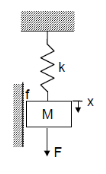
\includegraphics[scale=0.6]{images/p1.png}
\end{figure}

Recordando
\begin{itemize}
\item $\sum F=m*a$
\item $fricción = F*v$ (fuerza*velocidad)
\item $resistencia = F*x$ (fuerza*posición)
\end{itemize}

Al ser un sistema mecánico $\sum F=m*a$ donde:
\begin{itemize}
\item m es la masa
\item f es la fricción $f*v (fuerza*velocidad)$
\item F es la fuerza de entrada
\item k es la fuerza de la resistencia $k*x$ (resistencia*posición)
\item a es la segunda derivada de la posición
\end{itemize}

De esta forma, podemos representar el sistema como: $\sum F =$ Fuerza entrada - fricción - resistencia \\

$m*a = M\ddot{x}$ \\

$F - kx - f*\dot{x} = M\ddot{x}$ \\
$F_{entrada} - F_{k}*x - F_{fricción}*\frac{dx(t)}{dt} = M*\frac{d^2 x(t)}{dt}$ \\

teniendo asi: $F_{entrada} = M*\frac{d^2 x(t)}{dt} + F_{friccion} * \frac{dx(t)}{dt} + k*x$ \\

\newpage
Aplicando la Transformada de Laplace: \\
$F=f*\frac{d x(t)}{dt} + M * \frac{d^{2} x(t)}{dt} + k*x$ \\

$F(s) = fsX(s)+Ms^{2}X(s)+kX(s)$ \\

$F(s) = (fs+Ms^{2}+k)X(s)$ \\

$X(s) = \frac{F(s)}{Ms^{2}+fs+k}$ \\

\fbox{\begin{minipage}{15em}
$\frac{X(s)}{F(s)} = \frac{F(s)}{(Ms^2+fs+k)F(s)} = \frac{1}{Ms^2+fs+k}$
\end{minipage}}


\newpage
\section*{{\color{Apricot}Modelado 2}}

\begin{figure}[H]
  \centering
  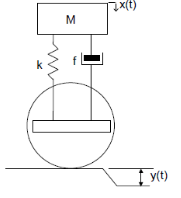
\includegraphics[scale=0.6]{images/p2.png}
\end{figure}

Sistema mecánico $\sum F=m*a$ \\

datos del sistema:
\begin{itemize}
\item k - $resistencia = F*v$ 
\item f - $amortiguador = F*posición$
\item m - $masa$
\item entrada del sistema - bache $y(t)$
\item salida del sistema - $x(t)$
\end{itemize}

$-F * \frac{d x(t)}{dt} - F_{posición} = m * \frac{d^2 x(t)}{dt}$ \\

$-k * \frac{d (x-y)}{dt} - f(x-y) = m * \frac{d^2 (x-y)}{dt}$ \\

$-k(\dot{x}-\dot{y})-f(x-y) = m*(\ddot{x}-\ddot{y})$ \\

Aplicando la transformada de Laplace \\

$-ksX(s)+ksY(s)-fX(s)+fY(s)=s^{2}mX(s)-s^{2}mY(s)$ \\ \\

reacomodando terminos \\
$ksY(s)+fY(s)+s^{2}mY(s) = ksX(s)+fX(s)+s^{2}mX(s)$ \\ \\

\fbox{\begin{minipage}{15em}
$\frac{Y(s)}{X(s)} = \frac{ks+f+s^{2}m}{ks+f+s^{2}m} = 1$
\end{minipage}}

\newpage
\section*{{\color{Apricot}Modelado 3}}

\begin{figure}[H]
  \centering
  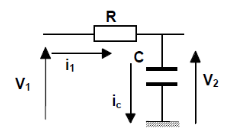
\includegraphics[scale=0.6]{images/p3.png}
\end{figure}

Filtro pasa bajas \\

La corriente de la malla $i_{R} = i_{C}$ ; El voltaje de salida $V_{2}$ coincide con el voltaje en el capacitor \\

$V_{C} = V_{2} = \frac{1}{C} \int i(t) dt$ ó para la corriente: \\

$i(t) = C \frac{d V_{2}(t)}{dt}$ \\

El voltaje en una malla cerrada es igual a la suma de sus caidas $V_{1} = V_{R} + V_{C}$ considerando que el voltaje de salida es el mismo que el capacitor $V_{1} = V_{R} + V_{2}$ \\

Expresando $V_{R}$ en función del voltaje de salida: $V_{R} = R*i$ , pero la corriente es la derivada del voltaje por la capacitancia presente \\

$V_{R} = R*C \frac{d V_{2}(t)}{dt}$ teniendo asi: \\

$V_{1} = R*C \frac{d V_{2}(t)}{dt} + V_{2}$ Obteniendo la transformada de Laplace \\

$V_{1}(s) = sRCV_{2}(s)+V_{2}(s) = (sRC+1)V_{2}(s)$ \\

\fbox{\begin{minipage}{15em}
$\frac{V_{2}(s)}{V_{1}(s)} = H(s) = \frac{1}{sRC+1}$
\end{minipage}}

\newpage
\section*{{\color{Apricot}Modelado 4}}

\begin{figure}[H]
  \centering
  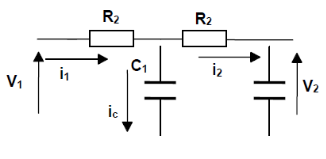
\includegraphics[scale=0.6]{images/p4.png}
\end{figure}

La variable de interes es el voltaje en el capacitor $C_{2}$ que es la salida del sistema $V_{2}$ \\

$V_{1} = V_{R1} + V_{C1}$ (1) \\

a su vez $V_{C1} = V_{R2} + V_{C2}$ (2) \\

Reemplazano $V_{C1}$ en (1) \\

$V_{1} = V_{R1} + V_{R2} + V_{C2}$ (3) encontrar $V_{R1}$ y $V_{R2}$ en función de su salida. \\

$V_{R1} = R_{1} * i_{1}$ (4)  y $V_{R2} = R_{2} * i_{2}$ (5) \\

Para el capacitor 2, dado que la corriente $i_{2}$ pasa por el Capacitor 2 la corriente que pasa por un capacitor esta dada por:\\

$i_{2} = C_{2} * \frac{d V_{C2}(t)}{dt}$ (6) sustituyendo en (5) \\

$V_{R2} = R2 * C_{2} \frac{d V_{C2}(t)}{dt}$ (7) \\

Para el Capacitor 1, la corriente que pasa en ese nodo es $i_{1} - i_{2} = C_{1} \frac{d V_{C1}(t)}{dt}$ (8) \\

despejando $i_1$ \\

$i_{1} = i_{2} + C_{1} \frac{d V_{C1}(t)}{dt}$ (9) \\

sustituyendo $i_{2}$ (6) en (9) \\

$i_{1} = C_{2} * \frac{d V_{C2}(t)}{dt} + C_{1} * \frac{d V_{C1}(t)}{dt}$ (10) \\

reemplazando $V_{C1}$ \\

$i_{1} = C_{2} * \frac{d V_{C2}(t)}{dt} + C_{1} * \left( \frac{d V_{R2}(t)}{dt} + \frac{d V_{C2}(t)}{dt} \right)$ (11) \\

$i_{1} = C_{2} * \frac{d V_{C2}(t)}{dt} + C_{1} * \left( R_{2}C_{2} \frac{d^{2}V_{C2}}{dt^{2}} + \frac{d V_{C2}(t)}{dt} \right)$ (12)\\

reemplazando en (4) \\

$V_{R1} = R_{1} * \left( C_{2} * \frac{d V_{C2}(t)}{dt} + C_{1}* \left( R_{2}C_{2} \frac{d^{2}V_{C2}(t)}{dt}+\frac{dV_{C2}}{dt} \right) \right)$ (13) \\

sustituyendo en la ecuación (3) \\

$V_{1} = R_{1}C_{1}R_{2}C_{2}*\frac{d^{2}V_{C2}(t)}{dt} + \left( R_{1}C_{1}+R_{1}C_{2}+R_{2}C_{2}\right) \frac{dV_{C2}}{dt} + V_{C2}$ \\

Agrupamos las constantes en terminos: \\

$a_{2} = R_{1}C_{1}R_{2}C_{2}$ \\
$a_{1} = R_{1}C_{2}+R_{1}C_{2}+R_{2}C_{2}$ \\

teniendo así: \\

$V_{1} = a_{2} \frac{d^{2}V_{C2}}{dt^{2}} + a_{1}*\frac{dV_{C1}}{dt} + V_{2}$ \\

Aplicando la transformada de Laplace \\

$V_{1}(s) = a_{2}s^{2}V_{2} + a_{1}sV_{2}(s) + V_{2}(s)$ \\

factorizando \\

$V_{1}(s) = (a_{2}s^{2}+a_{1}s+1)V_{2}(s)$ \\

Función de transferencia \\

$\frac{V_{2}(s)}{V_{1}(s)} =  \frac{1}{a_{2}s^{2}+a_{1}s+1}$ reemplazando las constantes tenemos: \\

\fbox{\begin{minipage}{25em}
$\frac{V_{2}(s)}{V_{1}(s)} = H(s) = \frac{1}{(R_{1}C_{1}R_{2}C_{2})s^{2}+(R_{1}C_{1}+R_{1}C_{2}+R_{2}C_{2})s+1}$
\end{minipage}}

\end{document}
